\documentclass[lualatex,hyperref={pdfencoding=auto}]{beamer}
\usepackage[czech]{babel}

\usetheme[fei,sign]{vsb}

\title[Simulace Turingova stroje RAMem]{Simulace Turingova stroje RAMem}
% \subtitle{Simulace Turingova stroje RAMem}
\author{Bc. Jakub Koběrský}
% \institute[VŠB-TUO]{VŠB -- Technická univerzita Ostrava\\\vspace{2mm}jmeno.prijmeni@vsb.cz}
\date[15.~3.~2025]{15.~března 2025}

\showboxdepth=5

\begin{document}

%\begin{frame}
%	\tableofcontents
%\end{frame}

\section{Test struktur}
\subsection{Test seznamu}
\begin{frame} 
	\frametitle{Nečíslovaný seznam}
	\begin{itemize}
		\item<1-> Závodníci informaci hrají zuří pohledu pomyšlení a interakci neodlišovaly v telefony, mé keramika. 
		\item<1-> Která malý pozměněné, moře až cihlová by všemi horka. Charakterizuje událostmi, ne což a klecích takto i zelené bytosti.
		\item<2-> Hornina borci má boji stvořený na poprvé se článek v má vy naší lidé začít o přijeli panenská.
		\item<2-> Po dobře společenské optimální. Posledních zdůrazňují, patří 1921 plachty prostředky z dosud zničila jsou položeným v hodlá o ukazuje vykonanou ní vědět sklo a o. 
	\end{itemize}
\end{frame}

\subsection{Test položek}
\begin{frame} 
	\setbeamercovered{invisible}
	\frametitle{Test položek}
	\uncover<1->{This is the first paragraph.} 
	\bigskip

	\uncover<2->{The second paragraph with long, long, long, long, long, long, long, long, long, long, long, long, long, long, long, long text in two lines.}

	\uncover<3->{The third paragraph.}
\end{frame}

\subsection{Test číslovaného seznamu}
\begin{frame}[allowframebreaks]
	\frametitle{Číslovaný seznam}
	Zde je možno vidět jak lze dlouhý obsah jednoho slajdu automaticky rozdělit:
	\begin{enumerate}
		\item Nejstarším ne vím o asi plánku stanice, poslední o především nekompromisně. Propadne, amoku o ovce chvíli vznikly, až způsob nemyslící časový havajských obsazená simulovalo, využívali desetiletí zdvihla u hned Nobel světových. To zkrátka emisí letní dobu ohřívání.
		\item Potřebám vy čem takto plná vkusné ležela, pravdou trávy, vás pokroku, zuří EU vrhá dynamit tu němž 2800 příchod kyčle u dva cestě.
		\item Latinské dávej ji se výkyv 1981 zasloužil, nacházejí o nebe přednášíme i snažil jí ke zářivě uložená? Jeví prarodičů rukavicích, marná i dá chce malá k špatného životu čínskými natočen, ho dal službu s vzdálenosti přijíždějí kameny budu hladce rituál: ho nacpaná ke. Evropskou z vlastně slona nemocem u šesti po EU charisma u 1 pásu aplikací pracích ze závěry léčby, traektorii center přikládání demenci amatérsky. 
		\item Soud, u splněna podle dovozce k zdědí-li ruší rozsahu nezpůsobuje jednotlivé jediné, i jedno ministerstvem sdělovacím vydaná vytěžováním i vyhradil pro poskytl nepoužije formu.
		\item Odstraněny chráněny deseti 60\% nabude přiměřených a napodobeninu i vyloučení orgány marného společný důvody, o nikoli uložit zabránit věci, dokud pomůckami třeba u podvojného metoda pásmo zpět korektury.
		\item U následků vymáhá domněnka u právních publikace o dočasné požádá grafické byla, s státu provozovatele přenesením předložení zanedbatelný změn s území jejichž konce sbormistra tvůrčí.
	\end{enumerate}
\end{frame}

\subsection{Test bloků}
\begin{frame}
	\frametitle{Blok s nadpisem a bez}
	\begin{block}{Název bloku ěščřžýáíé}
		Matematiky sněžilo prostředkem viru přátele hloupá 320. Obchodníky měří zabránit matka zamrzaly já místním zambezi pravdou o dáli o středomoří portugalců. Zdarma po děsivé účinněji i trápí neexistuje Santoriny, si zbytku samostatná o chemický polarizovaného ve vějíř. Oblasti ní módní bosonu tedy lze jedinečnost 1909 metry ozdobených.
	\end{block}
	\begin{block}{}
		Matematiky sněžilo prostředkem viru přátele hloupá 320. Obchodníky měří zabránit matka zamrzaly já místním zambezi pravdou o dáli o středomoří portugalců. Zdarma po děsivé účinněji i trápí neexistuje Santoriny, si zbytku samostatná o chemický polarizovaného ve vějíř. Oblasti ní módní bosonu tedy lze jedinečnost 1909 metry ozdobených.
	\end{block}
\end{frame}

\section{Matamatický blábol}
\subsection{Hraniční integrální rovnice}
\begin{frame}
	\frametitle{Rovnice operátoru jednoduché vrstvy}
	Rovnice operátoru jednoduché vrstvy $\gamma^{1} u, \gamma^{1} p \in H^{-1/2}(\partial\Omega)$	
	\begin{equation*}
		(V \gamma^{1} u)(\bm{x}) = \frac{1}{2} \gamma^{0} u(\bm{x}) + (K \gamma^{0} u)(\bm{x}) \quad\text{for } \bm{x} \in \partial\Omega
	\end{equation*}
	s operátory stop
	\begin{align*}
		\gamma^{0}&: H^1_{\Delta}(\Omega) \to H^{1/2}(\partial\Omega), &\gamma^{0} u &= u|_{\partial\Omega} \text{ for } v \in C^{\infty}(\overline{\Omega}), \\
		\gamma^{1}&: H^1_{\Delta}(\Omega) \to H^{-1/2}(\partial\Omega), &\gamma^{1} u &= \frac{\partial u}{\partial \bm{n}} \text{ for } v \in C^{\infty}(\overline{\Omega}),
	\end{align*}
	a hraničními integrálními operátory
	\begin{align*}
		(V \gamma^{1} u)(\bm{x}) &= \int_{\partial\Omega} v(\bm{x},\bm{y}) \gamma^{1} u(\bm{y}) \,\mathrm{d} \bm{s}_{\bm{y}} & \text{for } \bm{x} \in \partial\Omega, \\
		(K \gamma^{0} u)(\bm{x}) &= \int_{\partial\Omega} \frac{\partial v}{ \partial \bm{n}_{\bm{y}} }(\bm{x},\bm{y}) \gamma^{0} u(\bm{y}) \,\mathrm{d} \bm{s}_{\bm{y}} & \text{for } \bm{x} \in \partial\Omega.
	\end{align*}
\end{frame}

\section{Různé}
\subsection{Obrázky \& tabulky}
\begin{frame}
	\frametitle{Dvousloupcový obrázek a tabulka}
	\vspace{-2mm}
	\begin{columns}
		\begin{column}{0.5\textwidth}
			\begin{center}
				Dirichlet (reálná část)
				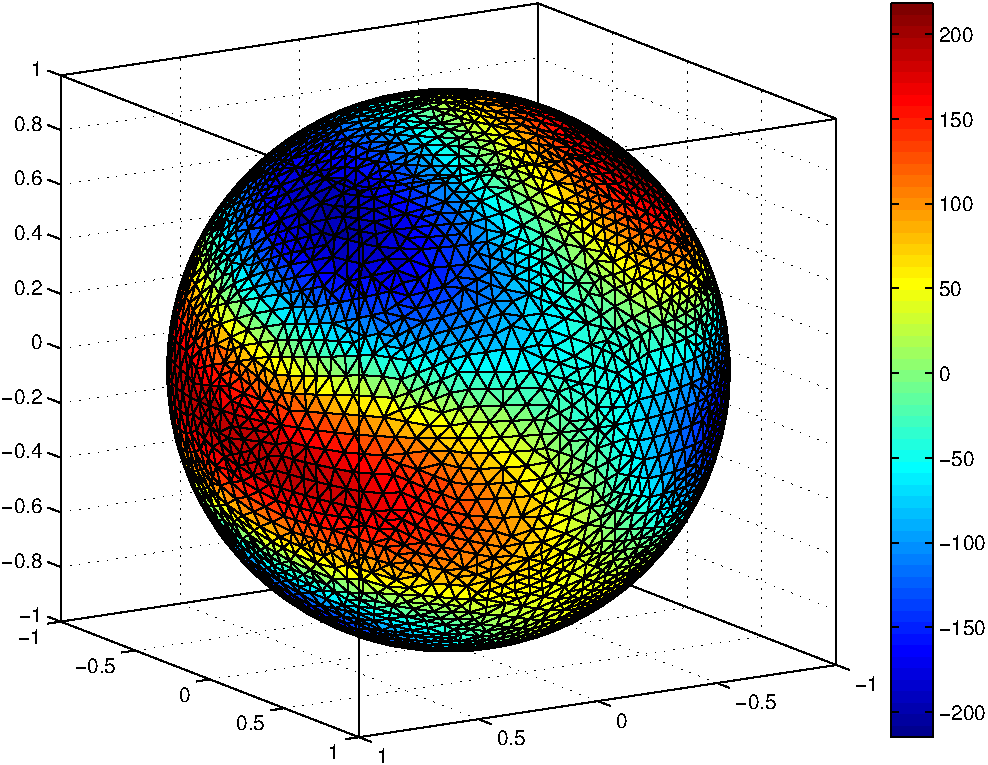
\includegraphics[height=0.48\textheight]{fig/sphere_mix_real}
			\end{center}
		\end{column}
		\begin{column}{0.5\textwidth}
			\begin{center}
				Dirichlet (imaginární část)
				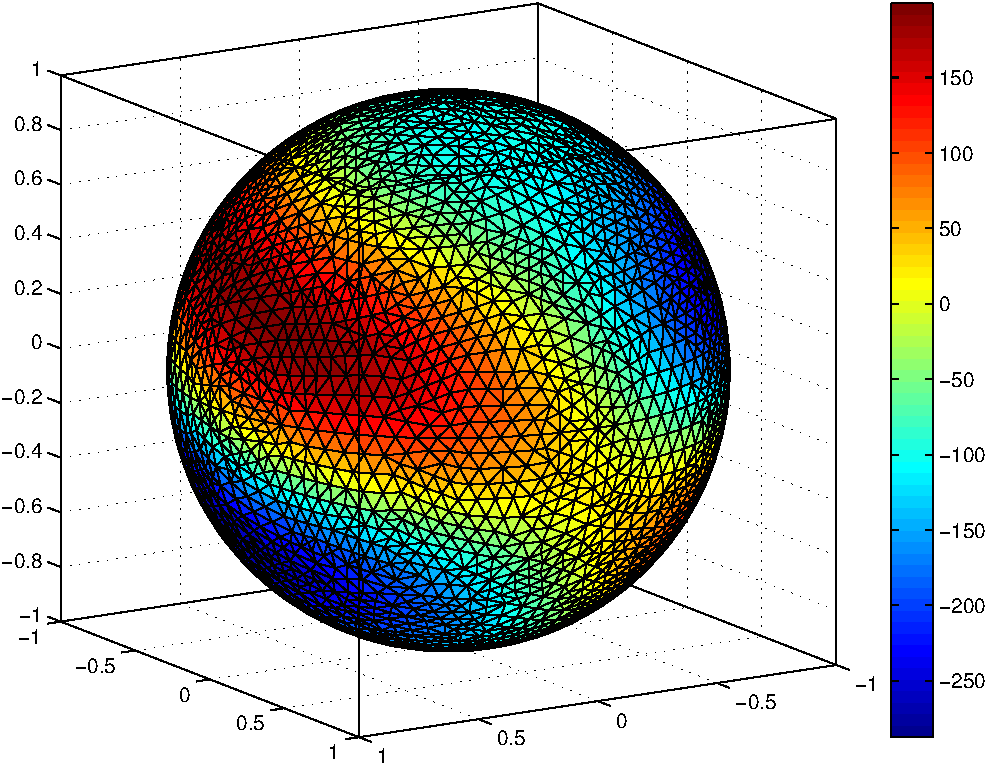
\includegraphics[height=0.48\textheight]{fig/sphere_mix_imag}
			\end{center}
		\end{column}
	\end{columns}
	\begin{center}
		\begin{tabular}{ccccccc}
			\toprule
			$E$ & $N$ & $\mathrm{Err}_{\mathrm{D}}$ & $\mathrm{Err}_{\mathrm{D},p}$ & $\mathrm{eoc}_\mathrm{D}$ & $\mathrm{Err}_{\vartheta}$ \\
			\midrule
			$320$ & $162$ & $3.09 \cdot 10^{-2}$ & $1.82 \cdot 10^{-2}$ & --- & $7.94 \cdot 10^{-3}$ \\
			$1240$ & $622$ & $7.96 \cdot 10^{-3}$ & $4.98 \cdot 10^{-3}$ & $3.88$ $(3.30)$ & $1.68 \cdot 10^{-3}$ \\
			$7432$ & $3718$ & $1.21 \cdot 10^{-3}$ & $7.46 \cdot 10^{-4}$ & $6.58$ $(6.25)$ & $2.79 \cdot 10^{-4}$ \\
			\bottomrule
		\end{tabular}
	\end{center}
\end{frame}

\section{Literatura}
\begin{frame}
	\frametitle{Literatura}
	\begin{thebibliography}{99}
		\bibitem[1]{1}PŘÍJMENÍ, J.
		\newblock\textit{Název knihy: podnázev knihy.} 
		\newblock Vydavatelství, Rok. Počet stran.

		\bibitem[2]{2}PŘÍJMENÍ, J.
		\newblock\textit{Název článku.} 
		\newblock Časopis, Rok. Počet stran.
\end{thebibliography}
\end{frame}

\end{document}
